\section{Results and Analysis}
\label{sec:results}

During the experiment programs' development, an automation mechanism was developed based on the GNU Make tool. This mechanism allowed for the repeated running of the experiments suite while also providing control over aspects such as the number of repetitions and grouping of the algorithms.

The basis for the mechanism was a series of additional rules added to the already-present ``Makefile'' files that had been developed for the building of each language's set of programs. A single target-rule, ``\texttt{experiments}'', would recursively descend into each language-specific directory and trigger all algorithms in sequence. Each algorithm ran a specified number of times, and in most cases the initial run was discarded. This was to prevent the possibility of the data input files being in the disk device's cache, skewing the timing and energy readings with regards to later runs. All non-error output from the experiments was captured by the harness program and streamed to a single text file.

The format chosen for the file of results was YAML, due to the ready availability of parsing libraries. YAML had an advantage over other formats such as CSV (comma-separated values) in that it allowed the flexibility of complex nested data were it to be necessary, while also being emitted in a streaming fashion. This greatly reduced the potential for output to be corrupted between algorithm executions.

\subsection{Results from the Experiments}
\label{subsec:results}

The automated suite of experiments was run numerous times over the course of this research. The final run from which the analysis and conclusions here are drawn is preserved in the same repository on the GitHub platform~\cite{github} as all the other files related to this research. The file of raw experiments data is named ``\texttt{experiments-data-20221111.yml}''. The final, full run of experiments took approximately 95 hours and 15 minutes to complete on the NUC device described in section~\ref{subsec:testing_platform}.

\subsubsection{Scope of the Experiments}

The final run of the experiments generated a total of 1,190 data-points taken from runs of the 30 programs. The set of programs below includes the regular expression variant of the DFA-Gap algorithm, as described in~\ref{subsubsec:dfa_regexp}. Table~\ref{table:iterations} shows the number of runs on a per-language, per-algorithm basis.

\begin{table}[h!]
\begin{center}
% Table: Algorithm iteration counts
% Generated: 2022-11-02 11:35:18.508914
\begin{tabular}{|c|c|c|c|c|c|c|}
\hline
Language&Knuth-Morris-Pratt&Boyer-Moore&Bitap&Aho-Corasick&DFA-Gap&Regexp-Gap \\
\hline
C (GCC)&25&25&25&25&10&n/a \\
C (LLVM)&25&25&25&25&10&n/a \\
C (Intel)&25&25&25&25&10&n/a \\
C++ (GCC)&25&25&25&25&10&n/a \\
C++ (LLVM)&25&25&25&25&10&n/a \\
C++ (Intel)&25&25&25&25&10&n/a \\
Rust&25&25&25&25&10&n/a \\
Perl&5&5&5&25&3&n/a \\
Python&5&5&5&25&3&n/a \\
\hline
\end{tabular}

\caption{Experiment iterations by language and algorithm}
\label{table:iterations}
\end{center}
\end{table}

For all numbers 10 and greater, there was an additional ``priming'' run (as described above) to ensure that disk cache status did not play into the values for full run-time or package-level energy usage. Note also that the DFA-Gap and Regexp-Gap columns are stand-ins for 5 such columns each (for the values of $k$ from 1 to 5). Each value of $k$ was run for the same number of iterations.

\subsubsection{Outliers and the Interpreted Languages}

While it was known that the interpreted languages (Python and Perl) would be slower than the compiled languages, the reality of the results was surprising: as will be shown in section~\ref{subsec:perf_comp}, below, the interpreted languages were in some cases more than 150 times slower than the fastest compiled program on the same algorithm.

This discovery required adjusting the automated experiments, to reduce the number of iterations for both interpreted languages. The Knuth-Morris-Pratt, Boyer-Moore, and Bitap algorithms were all reduced to 5 iterations each, for these languages. The Aho-Corasick algorithm ran in a more reasonable length of time and was left at 25 iterations, the same number as were run for the compiled languages.

For the DFA-Gap algorithm, both compiled and interpreted languages had to be reduced in terms of iterations given that approximate-matching algorithms are in general slower than their exact-matching counterparts. The compiled languages ran 5 iterations of this algorithm for values of $k$ ranging from 1 to 5, whereas the interpreted languages were necessarily limited to 3 iterations for the same values of $k$. When the regular expressions variant of the algorithm was added, it too was run for 5 and 3 iterations over the languages.

\subsection{Performance Comparisons}
\label{subsec:perf_comp}

The first of the three measures of the languages' suitability was chosen to be the overall performance. This was chosen for first consideration as this is the metric that most developers notice first: how long did it take the program to complete? Run-time measurement was also the easiest of the metrics to gather, both in terms of total program execution and in wall-clock time specifically spent in the algorithms themselves.

It was in the measuring of performance that it first became clear what a stark difference there was between the interpreted and compiled languages. One can forget the extent of this gap when working with interpreted languages in-depth for long periods of time. The Perl and Python performance numbers were so large in many cases that they had to be omitted from charts to preserve clarity, even when put to logarithmic scaling.

\subsubsection{Adjusting for Perl and Python}
\label{subsubsec:results:perf_perl_python}

Early examination of the performance results for Perl and Python (section~\ref{subsubsec:dfa_regexp}) had shown that the custom-built DFAs were strongly out-performed by using those languages' native support for regular expressions. Looking at these results separately from the rest of the experiments, the difference was considerable as is shown in figure~\ref{fig:graph:dfa_regexp_comp}.

\begin{figure}[h]
	\centering
	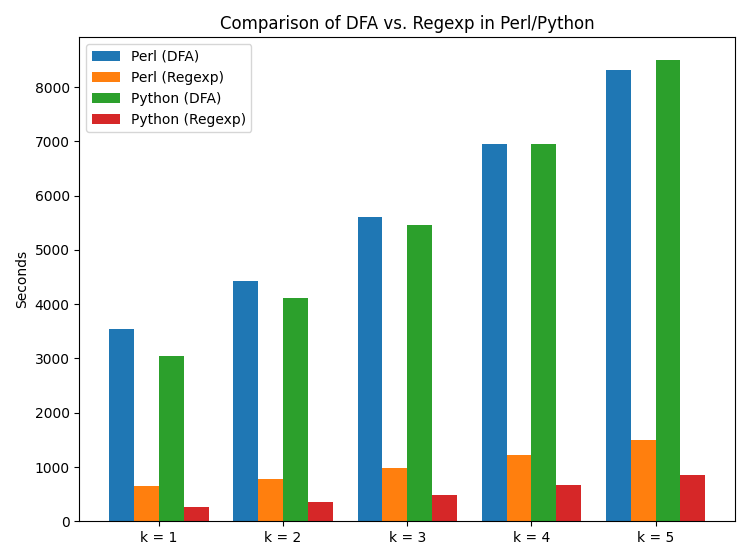
\includegraphics[width=0.85\textwidth]{figures/dfa_regexp_comp.png}
	\caption{Bar charts of DFA vs. Regexp run-times for Perl and Python}
	\label{fig:graph:dfa_regexp_comp}
\end{figure}

Not only were the run-times themselves higher for the DFA implementations, but the growth in run-time as $k$ increases was more pronounced for the DFA implementations than for the regular expression implementations. Note that while Perl's DFA was outperformed by Python's for the first two values of $k$, at $k=3$ it was slightly lower and was steadily improving over Python for both $k=4$ and $k=5$. However, in the regular expression implementation Python remained the better performer consistently.

This had led to a significant question during development regarding the measurement of performance for the algorithms: should the Perl and Python manually-coded DFA implementations be replaced by the regular expression implementations? It is highly unlikely that an experienced programmer in either of these two languages would choose to create the DFA manually when they could instead create a regular expression based on the pattern and a given value of $k$, in any case. When the performance is so drastically disparate it seems even less likely.

It was decided instead to implement the regular expression version of the experiment for the remaining three languages and include this in the final results and analysis. Figure~\ref{fig:graph:dfa_regexp_comp2} shows the run-time differences for these languages.

\begin{figure}[h]
	\centering
	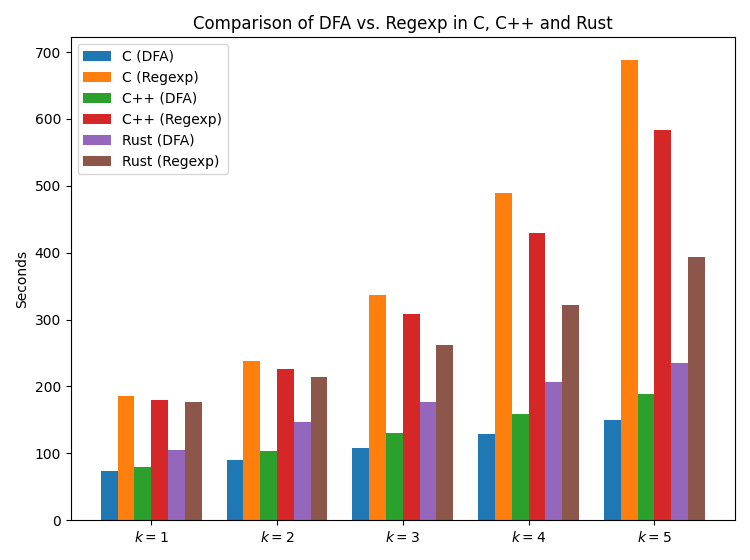
\includegraphics[width=0.85\textwidth]{figures/dfa_regexp_comp2.png}
	\caption{Bar charts of DFA vs. Regexp run-times for the compiled languages}
	\label{fig:graph:dfa_regexp_comp2}
\end{figure}

In these charts, the C and C++ values are averaged from the three toolchains. Examination of the complete run-time tables for DFA-Gap (\ref{table:runtime:dfa_gap:combined}) and Regexp-Gap (\ref{table:runtime:regexp:combined}) showed that each toolchains' run-times were extremely close to each other. This is understandable, as the majority of the work in these cases would have been done by the PCRE2 library itself which is identical across the different toolchain executables.

While regular expressions improved the performance of both Perl and Python dramatically, it did the reverse for the compiled languages. While C++ showed to be faster than C when using regular expressions and Rust faster still, as can be seen in figure~\ref{fig:graph:dfa_regexp_comp2} the use of regular expressions by the compiled languages took more time than the hand-crafted DFAs.

\subsubsection{Collected Performance Results}

After the decision was made to implement the regular expression variant throughout, processing of the full performance results was done. The collection of sub-tables in table~\ref{table:runtime:comparative-algorithm} shows the comparative performance of the languages on each of the algorithms. The time measurements are based on the algorithm run-time as opposed to the total run-time. In each table, the fastest language is listed first with the remaining ones following in order of performance. Run times are scaled by the fastest time. This has the result of showing each slower language's time as a percentage over the fastest. To obtain the run-time values used in the tables and charts, the mean run-times for each individual experiment were added together to represent each distinct language.

\begin{table}[!htb]
% Table: Comparative runtimes sub-tables
% Generated: 2022-11-12 18:00:26.811341
\begin{subtable}{0.33\textwidth}
    \centering
    \caption{Knuth-Morris-Pratt}
    \label{table:runtime:kmp}
    \begin{tabular}{|l|r|}
        %% Caption: Knuth-Morris-Pratt
        %% Label: table:runtime:kmp
        %% Field(s): ['runtime']
        \hline
        Language & Score \\
        \hline
        C (LLVM) & 1.0000 \\
        Rust & 1.1293 \\
        C++ (LLVM) & 1.1377 \\
        C (Intel) & 1.1402 \\
        C++ (Intel) & 1.2406 \\
        C (GCC) & 1.3146 \\
        C++ (GCC) & 1.3350 \\
        Perl & 38.5237 \\
        Python & 41.4858 \\
        \hline
    \end{tabular}
\end{subtable}%
\begin{subtable}{0.33\textwidth}
    \centering
    \caption{Boyer-Moore}
    \label{table:runtime:boyer_moore}
    \begin{tabular}{|l|r|}
        %% Caption: Boyer-Moore
        %% Label: table:runtime:boyer_moore
        %% Field(s): ['runtime']
        \hline
        Language & Score \\
        \hline
        C (Intel) & 1.0000 \\
        C++ (Intel) & 1.0508 \\
        C (GCC) & 1.0664 \\
        Rust & 1.0977 \\
        C++ (LLVM) & 1.1413 \\
        C (LLVM) & 1.1549 \\
        C++ (GCC) & 1.1831 \\
        Perl & 46.9470 \\
        Python & 50.9587 \\
        \hline
    \end{tabular}
\end{subtable}%
\begin{subtable}{0.33\textwidth}
    \centering
    \caption{Bitap}
    \label{table:runtime:shift_or}
    \begin{tabular}{|l|r|}
        %% Caption: Bitap
        %% Label: table:runtime:shift_or
        %% Field(s): ['runtime']
        \hline
        Language & Score \\
        \hline
        C (Intel) & 1.0000 \\
        C (GCC) & 1.0068 \\
        C++ (Intel) & 1.0475 \\
        C (LLVM) & 1.1219 \\
        Rust & 1.1350 \\
        C++ (GCC) & 1.1616 \\
        C++ (LLVM) & 1.2381 \\
        Perl & 155.3435 \\
        Python & 192.9283 \\
        \hline
    \end{tabular}
\end{subtable}
\begin{subtable}{0.33\textwidth}
    \centering
    \caption{Aho-Corasick}
    \label{table:runtime:aho_corasick}
    \begin{tabular}{|l|r|}
        %% Caption: Aho-Corasick
        %% Label: table:runtime:aho_corasick
        %% Field(s): ['runtime']
        \hline
        Language & Score \\
        \hline
        C (LLVM) & 1.0000 \\
        C (Intel) & 1.0443 \\
        C (GCC) & 1.0644 \\
        C++ (GCC) & 1.1519 \\
        C++ (LLVM) & 1.1600 \\
        Rust & 1.1816 \\
        C++ (Intel) & 1.1988 \\
        Python & 19.7040 \\
        Perl & 39.4041 \\
        \hline
    \end{tabular}
\end{subtable}%
\begin{subtable}{0.33\textwidth}
    \centering
    \caption{DFA-Gap (k=3)}
    \label{table:runtime:dfa_gap}
    \begin{tabular}{|l|r|}
        %% Caption: DFA-Gap (k=3)
        %% Label: table:runtime:dfa_gap
        %% Field(s): ['runtime']
        \hline
        Language & Score \\
        \hline
        C (GCC) & 1.0000 \\
        C (LLVM) & 1.0749 \\
        C (Intel) & 1.1561 \\
        C++ (GCC) & 1.2270 \\
        C++ (LLVM) & 1.3250 \\
        C++ (Intel) & 1.3443 \\
        Rust & 1.7632 \\
        Perl & 56.2209 \\
        Python & 57.4437 \\
        \hline
    \end{tabular}
\end{subtable}%
\begin{subtable}{0.33\textwidth}
    \centering
    \caption{Regexp-Gap (k=3)}
    \label{table:runtime:regexp}
    \begin{tabular}{|l|r|}
        %% Caption: Regexp-Gap (k=3)
        %% Label: table:runtime:regexp
        %% Field(s): ['runtime']
        \hline
        Language & Score \\
        \hline
        Rust & 1.0000 \\
        C++ (LLVM) & 1.1747 \\
        C++ (GCC) & 1.1753 \\
        C++ (Intel) & 1.1794 \\
        C (Intel) & 1.2871 \\
        C (GCC) & 1.2876 \\
        C (LLVM) & 1.2888 \\
        Python & 1.7398 \\
        Perl & 3.9966 \\
        \hline
    \end{tabular}
\end{subtable}

\caption{Comparative run-times by algorithm}
\label{table:runtime:comparative-algorithm}
\end{table}

The DFA-Gap and Regexp algorithms are shown for just $k=3$. However, there was some fluctuation in the ranking of the languages as $k$ went from 1 to 5. For the calculation of the metric of performance, all values of $k$ for both of these algorithms will be used.

The set of charts in figures~\ref{fig:graph:kmp-runtimes} to~\ref{fig:graph:regexp-runtimes} illustrate the run-times by language for each of the six algorithms. Note that all of these except figure~\ref{fig:graph:regexp-runtimes} omit the Perl and Python languages due to their extreme differences in the scale of running-time\footnote{As was mentioned, a logarithmic scale was also tried but the Perl/Python values were still too far from the norm (particularly in the Bitap results).}.

\begin{figure}[ht]
    \centering
    \begin{minipage}[t]{0.45\textwidth}
        \centering
        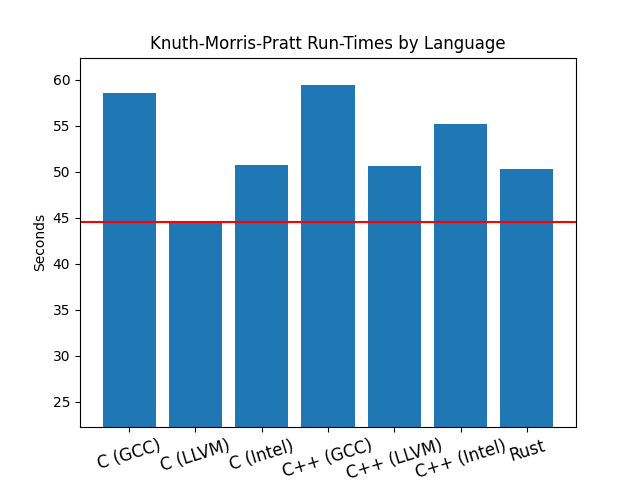
\includegraphics[width=0.85\textwidth]{figures/algorithm_runtimes-kmp.png}
        \caption[Knuth-Morris-Pratt run-times]{KMP run-times}
        \label{fig:graph:kmp-runtimes}
    \end{minipage}\hfill
    \begin{minipage}[t]{0.45\textwidth}
        \centering
        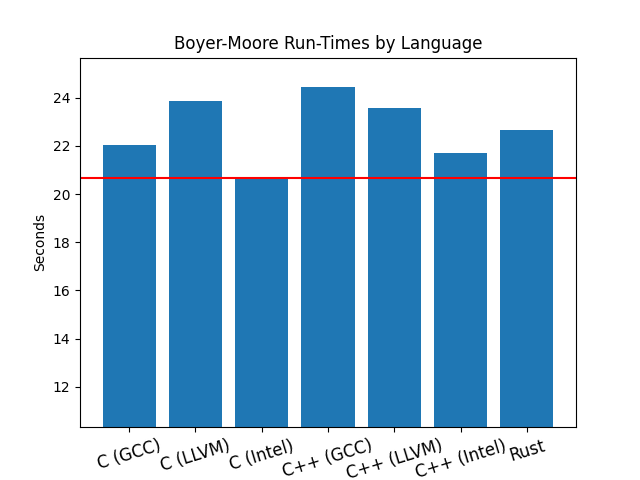
\includegraphics[width=0.85\textwidth]{figures/algorithm_runtimes-boyer_moore.png}
        \caption[Boyer-Moore run-times]{BM run-times}
        \label{fig:graph:bm-runtimes}
    \end{minipage}
\end{figure}

Starting with the Knuth-Morris-Pratt (\ref{fig:graph:kmp-runtimes}) and Boyer-Moore (\ref{fig:graph:bm-runtimes}) algorithms which have a passing relation to each other, the red lines indicate the fastest run-time and are meant to show the difference in the other languages' finish-time. In the Knuth-Morris-Pratt results, of interest is the fact that both C and C++ compiled by the LLVM toolchain strongly out-performed the GCC and Intel toolchains. This was the only algorithm in which LLVM controlled the performance for both languages. In Boyer-Moore, the Intel toolchain took the top spot with C, and the second spot with C++. Though this is not the only algorithm for which a C++ experiment placed second, this is the highest that C++ placed throughout all algorithms.

\begin{figure}[ht]
    \centering
    \begin{minipage}[t]{0.45\textwidth}
        \centering
        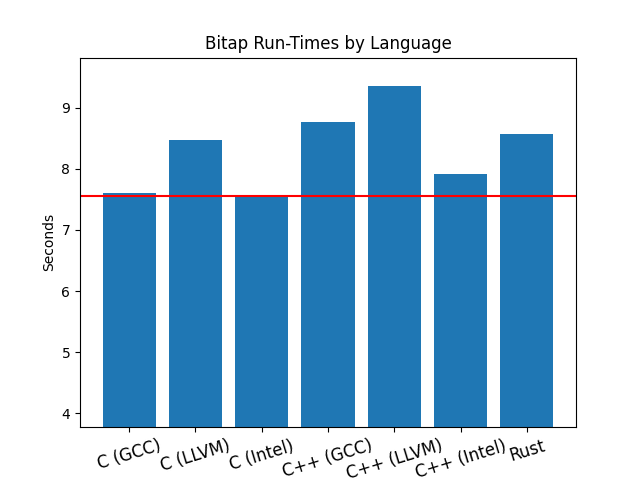
\includegraphics[width=0.85\textwidth]{figures/algorithm_runtimes-shift_or.png}
        \caption{Bitap run-times}
        \label{fig:graph:bitap-runtimes}
    \end{minipage}\hfill
    \begin{minipage}[t]{0.45\textwidth}
        \centering
        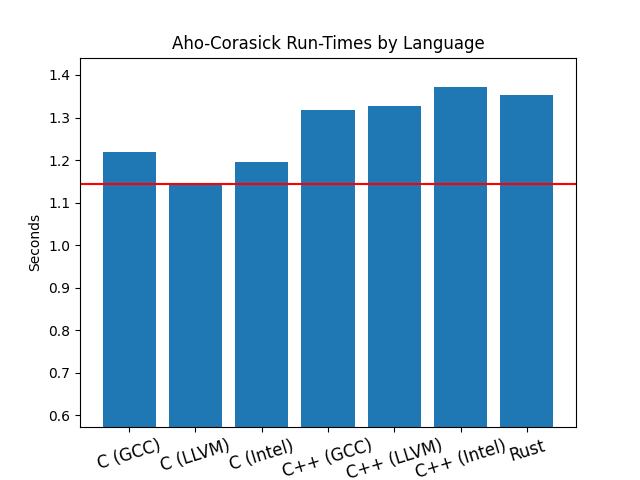
\includegraphics[width=0.85\textwidth]{figures/algorithm_runtimes-aho_corasick.png}
        \caption[Aho-Corasick run-times]{AC run-times}
        \label{fig:graph:ac-runtimes}
    \end{minipage}
\end{figure}

In the Bitap results shown in figure~\ref{fig:graph:bitap-runtimes}, the LLVM toolchain actually produced the slowest times within the C and C++ groups in this case. In the Aho-Corasick results (figure~\ref{fig:graph:ac-runtimes}) LLVM once again produced the fastest code for the C version of the experiment. The Aho-Corasick run-times also highlight the overall speed of this algorithm, enabled by the ability to test all patterns in a single pass through each target sequence.

\begin{figure}[ht]
    \centering
    \begin{minipage}[t]{0.45\textwidth}
        \centering
        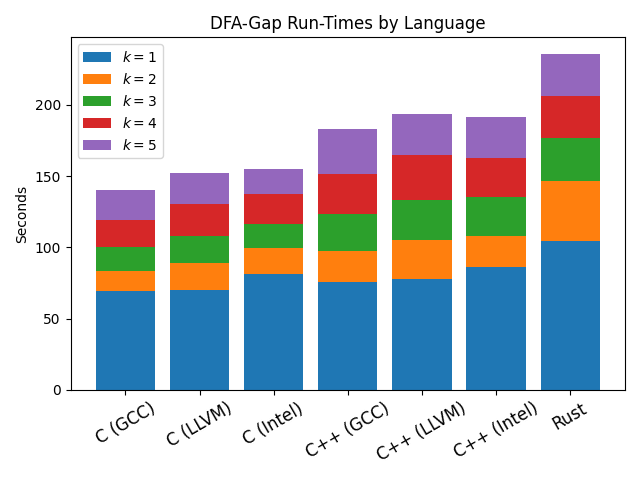
\includegraphics[width=0.85\textwidth]{figures/algorithm_runtimes-dfa_gap.png}
        \caption[DFA-Gap run-times]{DFA run-times}
        \label{fig:graph:dfa-runtimes}
    \end{minipage}\hfill
    \begin{minipage}[t]{0.45\textwidth}
        \centering
        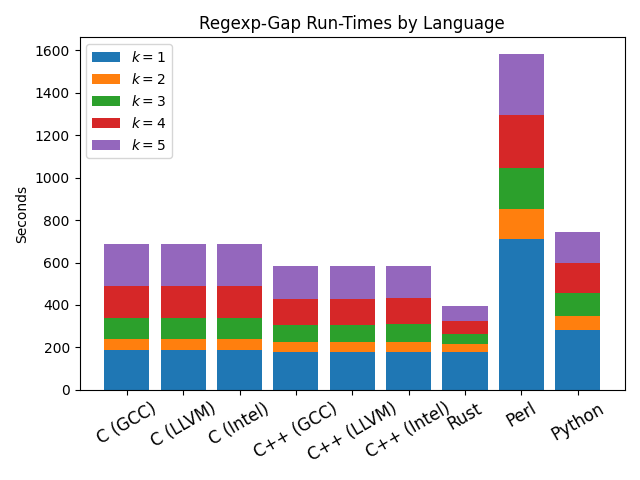
\includegraphics[width=0.85\textwidth]{figures/algorithm_runtimes-regexp.png}
        \caption[Regexp-Gap run-times]{Regexp run-times}
        \label{fig:graph:regexp-runtimes}
    \end{minipage}
\end{figure}

For the DFA and regular expression versions of the gap algorithm, figures~\ref{fig:graph:dfa-runtimes} and~\ref{fig:graph:regexp-runtimes}, different styles of charts were drawn. As both of these experiments ran for five different values of the $k$ parameter, the charts are designed to show all five run-times for each language as a stack.

The DFA experiments follow an almost expected trajectory, with C being faster than C++ and C++ faster than Rust. However, the regular expression experiments show an exactly opposite trend, with Rust being the fastest of the languages. Figure~\ref{fig:graph:regexp-runtimes} also includes results for the Perl and Python languages, as this experiment gave results for them that could be comfortably included.

Full tables of run-times scores for all values of $k$ in both DFA-Gap and Regexp-Gap experiments can be found in section~\ref{sec:extra_tables}. A short analysis of the relative size of the run-times themselves is done in section~\ref{sec:extra_graphs}, as those details are less directly relevant to the collected performance calculations.

\subsection{Expressiveness Comparisons}
\label{subsec:expr_comp}

Expressiveness was generally the most-challenging of the metrics to measure and evaluate. Even the most concrete, numerical measurements of code such as SLOC and complexity are subject to some debate and dissent. In these aspects of the research, measurement was taken through a range of open-source tools and the results tracked closely with expectation; the interpreted languages showed the strongest scores on the three expressiveness sub-metrics.

However, much of what was measured for this metric was also dependent upon the skill shown in the writing of the programs. Familiarity with the different languages varied, from significant experience in C and Perl to relative newness with regards to Rust. It is not possible to say whether someone more expert in the Rust language, for example, could have implemented the chosen algorithms with more efficiency and better expressiveness metrics.

Additionally, the complexity component of this metric had been cast in some doubt by the inability to use a single tool for all languages involved. This is shown in section~\ref{subsec:final-rankings} to have not influenced the final rankings.

In comparing expressiveness, it is useful to look at all three of the chosen comparative measures in an aggregated fashion. First, the individual numbers will be examined. As with the previous two bases, tables will show the numbers comparing the languages. Unlike the previous sections, the numbers shown will be for the combined files of all algorithm modules, as well as runner modules and input modules. For each language the source code was combined in a way that facilitated each of the metrics:

\begin{description}
\item[SLOC:] Total SLOC values for each language's files were combined. In the case of C and C++, this includes relevant lines from the header files for the runner and input modules.
\item[Complexity:] Each file's cyclomatic complexity values were computed on a per-function basis. Each module's function scores were averaged, and all modules' averages for a given language were summed together.
\item[Conciseness:] Using a method adapted from Bergmans, et al~\cite{bergmans}, each source code file for a given language was stripped of comments and then merged into a sort of ``archive'' using the standard ``\texttt{cat}'' command available on Linux. Each such resulting file was then compressed with the ``\texttt{xz}'' compression utility and the compression ratio recorded.
\end{description}

\subsubsection{Source Lines of Code}

In table~\ref{table:expr:sloc}, the SLOC totals are shown in three sub-tables: only the algorithm implementations, then the framework totals, and finally the combined totals of all lines.

\begin{table}[!htb]
% Table: Comparative SLOC totals sub-tables
% Generated: 2022-11-04 19:01:11.807483
\begin{subtable}{0.33\textwidth}
    \centering
    \begin{tabular}{|c|r|r|}
        \hline
        Language & Code & Score \\
        \hline
        Python & 257 & 1.0000 \\
        Perl & 354 & 1.3774 \\
        C++ & 368 & 1.4319 \\
        C & 473 & 1.8405 \\
        Rust & 507 & 1.9728 \\
        \hline
    \end{tabular}
    \caption{Algorithm lines}
    \label{table:sloc:algorithm}
\end{subtable}%
\begin{subtable}{0.33\textwidth}
    \centering
    \begin{tabular}{|c|r|r|}
        \hline
        Language & Support & Score \\
        \hline
        Python & 148 & 1.0000 \\
        Perl & 211 & 1.4257 \\
        C++ & 266 & 1.7973 \\
        Rust & 272 & 1.8378 \\
        C & 353 & 2.3851 \\
        \hline
    \end{tabular}
    \caption{Framework lines}
    \label{table:sloc:framework}
\end{subtable}%
\begin{subtable}{0.33\textwidth}
    \centering
    \begin{tabular}{|c|r|r|}
        \hline
        Language & All & Score \\
        \hline
        Python & 405 & 1.0000 \\
        Perl & 565 & 1.3951 \\
        C++ & 634 & 1.5654 \\
        Rust & 779 & 1.9235 \\
        C & 826 & 2.0395 \\
        \hline
    \end{tabular}
    \caption{Total of lines}
    \label{table:sloc:all}
\end{subtable}

\caption{Comparison of SLOC by language}
\label{table:expr:sloc}
\end{table}

Here Python is the clear leader, with Perl being 40\% larger in table~\ref{table:sloc:all}. C++ maintains the third-place ranking across all three sub-tables, and Rust edges out C in both the framework measurement and the total lines measurement. Rust's score in table~\ref{table:sloc:algorithm} likely suffered from the necessary mechanism that was used to pass and unpack pattern representation between a given algorithm's initialization function and the algorithm function itself. Compare the listings, below.

\begin{lstlisting}[language=C,caption={C unpacking of pattern data},label={lst:c_unpack}]
    int *pattern_count = (int *)pat_data[0];
    int *goto_fn = (int *)pat_data[1];
    int *failure_fn = (int *)pat_data[2];
    Set *output_fn = (Set *)pat_data[3];
\end{lstlisting}


\begin{lstlisting}[language=Rust,caption={Rust unpacking of pattern data},label={lst:rust_unpack},showstringspaces=false]
    let pattern_count = match &pat_data[0] {
        MultiPatternData::PatternCount(val) => val,
        _ => panic!("Incorrect value at pat_data slot 0"),
    };
    let goto_fn = match &pat_data[1] {
        MultiPatternData::PatternIntVecVec(val) => val,
        _ => panic!("Incorrect value at pat_data slot 1"),
    };
    let failure_fn = match &pat_data[2] {
        MultiPatternData::PatternUsizeVec(val) => val,
        _ => panic!("Incorrect value at pat_data slot 2"),
    };
    let output_fn = match &pat_data[3] {
        MultiPatternData::PatternTypeVec(val) => val,
        _ => panic!("Incorrect value at pat_data slot 3"),
    };
\end{lstlisting}


In this area, C and C++ each needed only one line per element passed (listing~\ref{lst:c_unpack}), while Rust required four\footnote{One of which was a closing-brace with a semicolon and might not have been counted by the \texttt{sloc} tool.} (listing~\ref{lst:rust_unpack}). This is a 12-line difference in just the Aho-Corasick implementation, so it can be understood how this could propagate through the other algorithm implementations.

By further comparison: both Python and Perl, having the native ability to pass arrays of differing types, needed only one line to unpack the pattern representations.

\subsubsection{Cyclomatic Complexity}
\label{subsubsec:complexity}

Table~\ref{table:expr:cyclomatic} shows a similar break-down of the cyclomatic complexity measurements: algorithms, framework, and combined total.

\begin{table}[!htb]
% Table: Comparative cyclomatic totals sub-tables
% Generated: 2022-11-12 18:00:26.813913
\begin{subtable}{0.33\textwidth}
    \centering
    \caption{Algorithms complexity}
    \label{table:cyclomatic:algorithm}
    \begin{tabular}{|c|r|r|}
        \hline
        Language & Total & Avg \\
        \hline
        Python & 76 & 19.57 \\
        C++ & 81 & 16.83 \\
        Perl & 106 & 26.97 \\
        C & 114 & 18.30 \\
        Rust & 132 & 17.97 \\
        \hline
    \end{tabular}
\end{subtable}%
\begin{subtable}{0.33\textwidth}
    \centering
    \caption{Framework complexity}
    \label{table:cyclomatic:framework}
    \begin{tabular}{|c|r|r|}
        \hline
        Language & Total & Avg \\
        \hline
        C++ & 43 & 10.75 \\
        Python & 47 & 9.90 \\
        Rust & 58 & 5.43 \\
        Perl & 61 & 12.90 \\
        C & 76 & 19.00 \\
        \hline
    \end{tabular}
\end{subtable}%
\begin{subtable}{0.33\textwidth}
    \centering
    \caption{Total complexity}
    \label{table:cyclomatic:total}
    \begin{tabular}{|c|r|r|}
        \hline
        Language & Total & Avg \\
        \hline
        Python & 123 & 29.47 \\
        C++ & 124 & 27.58 \\
        Perl & 167 & 39.87 \\
        C & 190 & 37.30 \\
        Rust & 190 & 23.40 \\
        \hline
    \end{tabular}
\end{subtable}

\caption{Comparison of complexity by language}
\label{table:expr:cyclomatic}
\end{table}

Unlike the SLOC measurements, however, there is greater variation in the rankings of the languages. Here the contest between the first and second rankings was between Python and C++. Rust placed last in the measure of the algorithm code, possibly due to the same issue of excess lines around the unpacking of pattern data. Rust did rank third in the framework table~\ref{table:cyclomatic:framework} where it also had a significantly lower average value than C++ or Python. Even as Rust ended tied for the fourth rank in the total table, its totaled average complexity was still the lowest of the five.

It is important here to note again that it was necessary to use different tools to calculate the complexity of the Perl and Rust code. The \texttt{lizard} tool did not support Perl at all, and examination of the Rust results showed some bugs in the handling of Rust. Because of this, it is not possible to say with certainty that the relative comparisons of complexity between the five languages are completely sound.

\subsubsection{Conciseness}
\label{subsubsec:conciseness}

Conciseness proved to be a difficult concept to quantify. The approach taken in~\cite{bergmans} was designed around a significantly larger database of source code, but as the results from that paper were compelling, it led to the adaptation of a variation of that methodology here.

The steps for deriving this measurement were:

\begin{enumerate}
\item A clean copy of all source code was made into a series of directories named by language
\item All comments and blank lines were removed by the \texttt{cloc} tool
\item Each individual language directory had all text files concatenated into a single file
\item Each of these text files were compressed with \texttt{xv} and the compression ratio recorded
\end{enumerate}

A key difference between~\cite{bergmans} and here is the limited scope of the data being analyzed; since there is essentially just one ``project'' being put to scrutiny, the results are sensitive to the fact that some of the files were smaller in size to begin with. Initially the technique in~\cite{bergmans} was followed exactly, and involved using the standard \texttt{tar} utility to create the archives of each language. But when put into practice it was found that the metadata overhead of a \texttt{tar} archive was more than the size of the actual data in some cases.

Further, in their paper, Bergmans and their team had removed most smaller examples of code for each language from the final measurements. This was not an option here given the limited size and number of the samples. For this reason the decision was made to focus the compression on the text content only, by applying concatenation to the stripped versions of the source files and compressing the results of this process.

In table~\ref{table:expr:compression}, the results are shown.

\begin{table}[!htb]
% Table: Compression ratios table
% Generated: 2022-11-11 19:03:08.366214
\centering
\begin{tabular}{|l|c|c|}
    \hline
    Language & Ratio & Score \\
    \hline
    Python & 78.50\% & 1.0000 \\
    Perl & 80.50\% & 1.0255 \\
    C & 80.60\% & 1.0268 \\
    Rust & 80.80\% & 1.0293 \\
    C++ & 81.00\% & 1.0318 \\
    \hline
\end{tabular}

\caption{Comparison of compressibility by language}
\label{table:expr:compression}
\end{table}

The ranking of Python and Perl as the first two is expected. However, the placing of C ahead of both Rust and C++ came as a surprise given the presence of highly-repetitive calls to library routines for the manual memory management. However, C and Rust both likely benefited from the need for additional support code in the Aho-Corasick algorithm which could have brought the compression ratio slightly further down.

\subsubsection{Combining the Expressiveness Metrics}

At this point the next step was to derive a single measurement of expressiveness from the three measurements taken. For this, it would be needed to have ``score'' values for cyclomatic complexity that were in line with the scores computed for SLOC and conciseness. These values were computed from table~\ref{table:cyclomatic:total} and are shown in table~\ref{table:expr:cyclomatic-score}.

\begin{table}[!htb]
% Table: Cyclomatic scores for all files
% Generated: 2022-11-11 19:03:08.367054
\centering
\begin{tabular}{|l|r|r|}
    \hline
    Language & Total & Score \\
    \hline
    Python & 123 & 1.0000 \\
    C++ & 124 & 1.0081 \\
    Perl & 167 & 1.3577 \\
    C & 190 & 1.5447 \\
    Rust & 190 & 1.5447 \\
    \hline
\end{tabular}

\caption{Scoring of the cyclomatic complexity results}
\label{table:expr:cyclomatic-score}
\end{table}

Here, the score shows a virtual tie for first position between C++ and Python. Their gap is just one point (less than 1\%), while the next gap is 43 (an increase of almost 35\%).

Now it would be possible to utilize the three expressiveness metrics to calculate a single value for each language. The following values would be combined into a series of 3-element vectors for each language:

\begin{itemize}
\item The SLOC scores from table~\ref{table:sloc:all}, the total of lines
\item The cyclomatic scores from table~\ref{table:expr:cyclomatic-score}
\item The conciseness scores from table~\ref{table:expr:compression}
\end{itemize}

The vectors were normalized into unit vectors. Then the vectors' lengths were calculated and scaled by the lowest value, giving the values in table~\ref{table:expr:expressiveness-score}:

\begin{table}[!htb]
% Table: Calculated expressiveness score
% Generated: 2022-11-07 19:21:37.618600
\centering
\begin{tabular}{|l|r|r|r|r|}
    \hline
    \thead{Language} & \thead{SLOC} & \thead{Complexity} & \thead{Compression} & \thead{Score} \\
    \hline
    Python & 1.0000 & 1.0000 & 1.0000 & 1.0000 \\
    C++ & 1.6000 & 1.0081 & 1.0318 & 1.1565 \\
    Perl & 1.3976 & 1.3577 & 1.0255 & 1.2109 \\
    Rust & 1.9405 & 1.5447 & 1.0293 & 1.4086 \\
    C & 2.0976 & 1.5447 & 1.0268 & 1.4503 \\
    \hline
\end{tabular}

\caption{Calculated expressiveness score}
\label{table:expr:expressiveness-score}
\end{table}

It was not a surprise that Python ended up ranked as the most-expressive of the five contenders, as it had led the group in all three expressiveness metrics. The ranking of C++ ahead of Perl by just over 5 percentage points was more of a surprise, while the presence of C at the bottom was not surprising.

Figure~\ref{fig:graph:expressiveness-arrows} illustrates the expressiveness values as vectors anchored at the origin. Judging the length of the vectors helps to show the difference between Python in the \nth{1} position and C in the \nth{5}.

\begin{figure}[h]
	\centering
    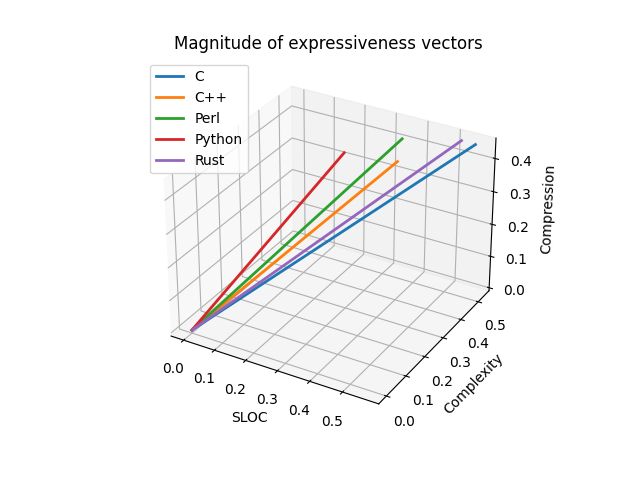
\includegraphics[width=0.85\textwidth]{figures/expressiveness_arrows.png}
    \caption{Calculated expressiveness as vectors}
    \label{fig:graph:expressiveness-arrows}
\end{figure}

Because of the possibly-inconsistent nature of the complexity data, it was decided to derive a second score based on just the SLOC and compression scores. All other calculation steps were the same. This resulted in table~\ref{table:expr:expressiveness-score2}.

\begin{table}[!hb]
% Table: Calculated expressiveness score (2-axis)
% Generated: 2022-11-11 19:03:10.009923
\centering
\begin{tabular}{|l|r|r|r|}
    \hline
    \thead{Language} & \thead{SLOC} & \thead{Compression} & \thead{Score} \\
    \hline
    Python & 1.0000 & 1.0000 & 1.0000 \\
    Perl & 1.3976 & 1.0255 & 1.1406 \\
    C++ & 1.6000 & 1.0318 & 1.2159 \\
    Rust & 1.9405 & 1.0293 & 1.3446 \\
    C & 2.0976 & 1.0268 & 1.4070 \\
    \hline
\end{tabular}

\caption{Calculated expressiveness score, 2-axis}
\label{table:expr:expressiveness-score2}
\end{table}

Here, the results more closely tracked with expectations: Python and Perl head the list while C++ and Rust take the next two places. As has been mentioned, it is possible that Rust suffered in the measurements due to the data-unpacking mechanism required by the framework.

\subsection{Energy Usage Comparisons}
\label{subsec:energy_comp}

In this section the energy usage results are examined. Table~\ref{table:energy:comparative-algorithm} shows the comparative energy usage over time (Joules per second) for each algorithm with the same scaling methodology applied as was used for the performance tables. The tables here use the ``Package'' and ``DRAM'' energy values combined together, divided by total run-time.

In regards to energy usage, the only significant barrier to overcome was ensuring that the machine used to run the experiments would be sufficiently isolated so as to have the least amount of interference possible from other running processes. The nature of the RAPL system of measuring power consumption also required that the experiments be run with super-user access levels. This amplified the need for the code to be as safe as possible, even though the testing machine was not made accessible to the general internet.

RAPL posed other challenges to use, such as the previously-mentioned 32-bit limitation in the registers used for tracking the energy usage. But this was overcome, and the RAPL system ended up proving robust-enough to handle measuring programs whose run-times ranged from barely one second to nearly three hours.

\begin{table}[!htb]
% Table: Comparative energy usage sub-tables
% Generated: 2022-11-11 19:03:08.364288
\begin{subtable}{0.33\textwidth}
    \centering
    \caption{Knuth-Morris-Pratt}
    \label{table:energy:kmp}
    \begin{tabular}{|l|r|}
        %% Caption: Knuth-Morris-Pratt
        %% Label: table:energy:kmp
        %% Field(s): ['package', 'dram']
        %% Divisor(s): ['total_runtime']
        \hline
        Language & Score \\
        \hline
        Rust & 1.0000 \\
        C (GCC) & 1.0403 \\
        C (LLVM) & 1.0756 \\
        C (Intel) & 1.0786 \\
        C++ (GCC) & 1.0983 \\
        C++ (LLVM) & 1.1033 \\
        C++ (Intel) & 1.1102 \\
        Python & 1.1651 \\
        Perl & 1.2957 \\
        \hline
    \end{tabular}
\end{subtable}%
\begin{subtable}{0.33\textwidth}
    \centering
    \caption{Boyer-Moore}
    \label{table:energy:boyer_moore}
    \begin{tabular}{|l|r|}
        %% Caption: Boyer-Moore
        %% Label: table:energy:boyer_moore
        %% Field(s): ['package', 'dram']
        %% Divisor(s): ['total_runtime']
        \hline
        Language & Score \\
        \hline
        C++ (GCC) & 1.0000 \\
        C++ (LLVM) & 1.0115 \\
        Rust & 1.0331 \\
        C (GCC) & 1.0358 \\
        C++ (Intel) & 1.0747 \\
        C (LLVM) & 1.0918 \\
        C (Intel) & 1.1501 \\
        Python & 1.2985 \\
        Perl & 1.3103 \\
        \hline
    \end{tabular}
\end{subtable}%
\begin{subtable}{0.33\textwidth}
    \centering
    \caption{Bitap}
    \label{table:energy:shift_or}
    \begin{tabular}{|l|r|}
        %% Caption: Bitap
        %% Label: table:energy:shift_or
        %% Field(s): ['package', 'dram']
        %% Divisor(s): ['total_runtime']
        \hline
        Language & Score \\
        \hline
        C++ (LLVM) & 1.0000 \\
        C (Intel) & 1.0049 \\
        Rust & 1.0077 \\
        C (LLVM) & 1.0101 \\
        C++ (Intel) & 1.0440 \\
        Python & 1.0799 \\
        C++ (GCC) & 1.0854 \\
        C (GCC) & 1.0897 \\
        Perl & 1.2268 \\
        \hline
    \end{tabular}
\end{subtable}
\begin{subtable}{0.33\textwidth}
    \centering
    \caption{Aho-Corasick}
    \label{table:energy:aho_corasick}
    \begin{tabular}{|l|r|}
        %% Caption: Aho-Corasick
        %% Label: table:energy:aho_corasick
        %% Field(s): ['package', 'dram']
        %% Divisor(s): ['total_runtime']
        \hline
        Language & Score \\
        \hline
        C++ (LLVM) & 1.0000 \\
        C (Intel) & 1.0303 \\
        C (GCC) & 1.0332 \\
        C (LLVM) & 1.0448 \\
        C++ (Intel) & 1.0471 \\
        C++ (GCC) & 1.0813 \\
        Rust & 1.0939 \\
        Perl & 1.1248 \\
        Python & 1.1736 \\
        \hline
    \end{tabular}
\end{subtable}%
\begin{subtable}{0.33\textwidth}
    \centering
    \caption{DFA-Gap (k=3)}
    \label{table:energy:dfa_gap(3)}
    \begin{tabular}{|l|r|}
        %% Caption: DFA-Gap (k=3)
        %% Label: table:energy:dfa_gap(3)
        %% Field(s): ['package', 'dram']
        %% Divisor(s): ['total_runtime']
        \hline
        Language & Score \\
        \hline
        Rust & 1.0000 \\
        C++ (LLVM) & 1.1603 \\
        C (LLVM) & 1.1812 \\
        C++ (Intel) & 1.2078 \\
        C (Intel) & 1.2231 \\
        C (GCC) & 1.2352 \\
        C++ (GCC) & 1.2497 \\
        Python & 1.3140 \\
        Perl & 1.3897 \\
        \hline
    \end{tabular}
\end{subtable}%
\begin{subtable}{0.33\textwidth}
    \centering
    \caption{Regexp-Gap (k=3)}
    \label{table:energy:regexp(3)}
    \begin{tabular}{|l|r|}
        %% Caption: Regexp-Gap (k=3)
        %% Label: table:energy:regexp(3)
        %% Field(s): ['package', 'dram']
        %% Divisor(s): ['total_runtime']
        \hline
        Language & Score \\
        \hline
        C (Intel) & 1.0000 \\
        C (GCC) & 1.0055 \\
        C (LLVM) & 1.0094 \\
        C++ (LLVM) & 1.0428 \\
        C++ (GCC) & 1.0460 \\
        C++ (Intel) & 1.0473 \\
        Perl & 1.0513 \\
        Rust & 1.0561 \\
        Python & 1.0618 \\
        \hline
    \end{tabular}
\end{subtable}

\caption{Comparative energy usage over time by algorithm}
\label{table:energy:comparative-algorithm}
\end{table}

The language exhibiting the lowest energy usage is listed first, with the rest ranked behind it. The DFA-Gap and Regexp algorithms are again represented by $k=3$, and again the rankings of the languages varied with $k$.

These results are further illustrated by figure~\ref{fig:graph:power_per_sec}. In this collection of bar-charts, the Rust language (represented by the pink bars) can be seen to be the lowest value in the Knuth-Morris-Pratt and DFA-Gap instances. In fact, Rust scored the lowest energy usage for all five variations of the DFA-Gap algorithm, making it the most-efficient language for 6 of the 14 distinct groups of experiments. Here, Perl and Python are included because the per-second measurements normalize their higher energy usage.

\begin{figure}[h]
	\centering
    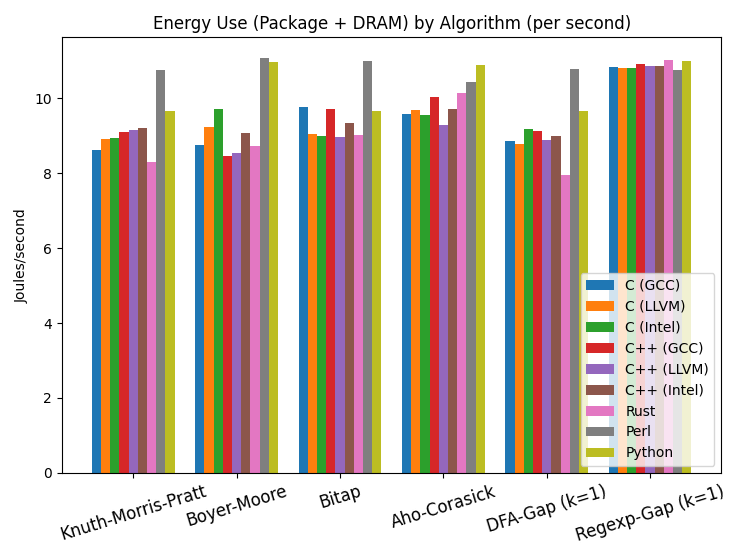
\includegraphics[width=0.85\textwidth]{figures/power_per_sec.png}
    \caption{Energy/second, by algorithm}
    \label{fig:graph:power_per_sec}
\end{figure}

The fact that Rust was the overall best performer in terms of energy usage is underscored by the chart in figure~\ref{fig:graph:total_power_usage}. In this chart, the value for each language as shown is the total of the mean values from all 14 experiments. Here, the Perl and Python languages have been removed again due to the fact that their longer run-times lead to energy numbers well out of scale with respect to the compiled languages. The red horizontal line shows the total usage by Rust and illustrates the differences with C and C++ across all three of their toolchains.

\begin{figure}[h]
	\centering
    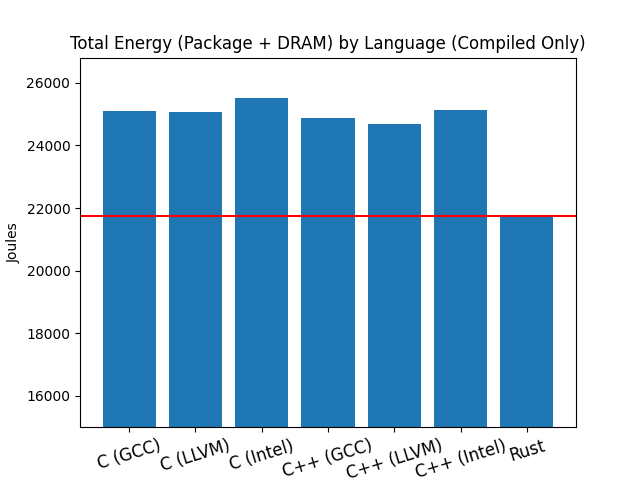
\includegraphics[width=0.85\textwidth]{figures/total_power_usage.png}
    \caption{Total energy by language}
    \label{fig:graph:total_power_usage}
\end{figure}

As with the run-times score tables, full tables of energy scores for all values of $k$ in both DFA-Gap and Regexp-Gap experiments can be found in section~\ref{sec:extra_tables}.

\subsection{Combining the Bases}
\label{subsec:combined}

With three distinct measurements available for combination and analysis, the first step was to derive a single set of scores for the run-time basis and the energy-used basis, combining the values from all 14 groups of experiments into single values. For this, values were simply added together then scaled by the minimum value as has been done before. The total run-time table~\ref{table:total:runtime} shows these values, derived from the algorithm-only run-time metric. In table~\ref{table:total:energy}, the same is done with the combination of the ``Package'' and ``DRAM'' energy metrics.

\begin{table}[!htb]
% Table: Total runtime and energy scores
% Generated: 2022-11-11 19:03:10.010647
\begin{subtable}{0.49\textwidth}
    \centering
    \caption{Scores for total run-time}
    \label{table:total:runtime}
    \begin{tabular}{|l|r|}
        \hline
        \thead{Language} & \thead{Score} \\
        \hline
        Rust & 1.0000 \\
        C++ (GCC) & 1.0561 \\
        C++ (LLVM) & 1.0694 \\
        C++ (Intel) & 1.0766 \\
        C (GCC) & 1.0947 \\
        C (LLVM) & 1.1056 \\
        C (Intel) & 1.1226 \\
        Python & 15.7236 \\
        Perl & 16.4693 \\
        \hline
    \end{tabular}
\end{subtable}%
\begin{subtable}{0.49\textwidth}
    \centering
    \caption{Scores for total energy usage}
    \label{table:total:energy}
    \begin{tabular}{|l|r|}
        \hline
        \thead{Language} & \thead{Score} \\
        \hline
        Rust & 1.0000 \\
        C++ (LLVM) & 1.1349 \\
        C++ (GCC) & 1.1435 \\
        C (LLVM) & 1.1525 \\
        C (GCC) & 1.1544 \\
        C++ (Intel) & 1.1551 \\
        C (Intel) & 1.1734 \\
        Python & 16.4127 \\
        Perl & 18.0492 \\
        \hline
    \end{tabular}
\end{subtable}

\caption{Final scores for totaled run-time and energy, by language}
\label{table:totals:runtime-energy}
\end{table}

From here came a question in two parts: Should the final scoring be based on the languages' scores for these bases or based on the language rankings? And secondly, should the cyclomatic complexity data be included in the expressiveness basis or not?

While the question regarding the complexity data has already been discussed, it still remained to be seen whether it would affect the final rankings. More than this, however, was the question of whether to simply apply the ranking of each language to determine final placement. Doing so might create a stronger distinction between adjacent languages than the scores themselves would. On the other hand, using the scores would retain the subtlety in the differences between languages.

The decision was made to examine all combinations of these two variables. Table~\ref{table:totals:all_metrics} shows the four sub-tables that result from this analysis. As can be seen from comparing \ref{table:final:scale_and_cc} with \ref{table:final:scale_no_cc}, and \ref{table:final:rank_and_cc} with \ref{table:final:rank_no_cc}, the cyclomatic complexity values did not affect the respective rankings at all: both pairs of tables have identical placement for their 9 rows. Comparing column-wise (\ref{table:final:scale_and_cc} with \ref{table:final:rank_and_cc}, and \ref{table:final:scale_no_cc} with \ref{table:final:rank_no_cc}), it can be seen that using the rank in place of scores lead to a slight difference in final ranking. Specifically, Rust and Python each moved up one place under a ranking basis. More significant, though, is how the different approaches affected the changes in scores.

\begin{table}[!htb]
% Table: Total scores tables
% Generated: 2022-11-11 19:03:10.010924
\begin{subtable}{0.49\textwidth}
    \centering
    \caption{Score by scale, with complexity}
    \label{table:final:scale_and_cc}
    \begin{tabular}{|l|r|}
        \hline
        \thead{Language} & \thead{Score} \\
        \hline
        C++ (GCC) & 1.0000 \\
        C++ (LLVM) & 1.0001 \\
        C++ (Intel) & 1.0007 \\
        Rust & 1.2058 \\
        C (GCC) & 1.2446 \\
        C (LLVM) & 1.2447 \\
        C (Intel) & 1.2454 \\
        Python & 3.2200 \\
        Perl & 3.4881 \\
        \hline
    \end{tabular}
\end{subtable}%
\begin{subtable}{0.49\textwidth}
    \centering
    \caption{Score by scale, no complexity}
    \label{table:final:scale_no_cc}
    \begin{tabular}{|l|r|}
        \hline
        \thead{Language} & \thead{Score} \\
        \hline
        C++ (GCC) & 1.0000 \\
        C++ (LLVM) & 1.0001 \\
        C++ (Intel) & 1.0006 \\
        Rust & 1.0987 \\
        C (GCC) & 1.1521 \\
        C (LLVM) & 1.1523 \\
        C (Intel) & 1.1529 \\
        Python & 3.0424 \\
        Perl & 3.2800 \\
        \hline
    \end{tabular}
\end{subtable}
\begin{subtable}{0.49\textwidth}
    \centering
    \caption{Score by ranks, with complexity}
    \label{table:final:rank_and_cc}
    \begin{tabular}{|l|r|}
        \hline
        \thead{Language} & \thead{Score} \\
        \hline
        C++ (GCC) & 1.0000 \\
        C++ (LLVM) & 1.0000 \\
        Rust & 1.4951 \\
        C++ (Intel) & 1.8150 \\
        C (GCC) & 2.4132 \\
        C (LLVM) & 2.4375 \\
        Python & 2.7547 \\
        C (Intel) & 2.9406 \\
        Perl & 3.3166 \\
        \hline
    \end{tabular}
\end{subtable}%
\begin{subtable}{0.49\textwidth}
    \centering
    \caption{Score by ranks, no complexity}
    \label{table:final:rank_no_cc}
    \begin{tabular}{|l|r|}
        \hline
        \thead{Language} & \thead{Score} \\
        \hline
        C++ (GCC) & 1.0000 \\
        C++ (LLVM) & 1.0000 \\
        Rust & 1.3143 \\
        C++ (Intel) & 1.6652 \\
        C (GCC) & 2.1213 \\
        C (LLVM) & 2.1426 \\
        Python & 2.4215 \\
        C (Intel) & 2.5849 \\
        Perl & 2.7469 \\
        \hline
    \end{tabular}
\end{subtable}

\caption{Final scores for all combined metrics, by language}
\label{table:totals:all_metrics}
\end{table}

Comparing the two sub-tables that include complexity values, it can be seen that the difference between the top (GCC C++) and bottom (Perl) is slightly higher in \ref{table:final:scale_and_cc} than in \ref{table:final:rank_and_cc}. This difference is even more pronounced in the two non-complexity tables.

\subsection{Confidence Intervals of the Data}
\label{subsec:confidence-intervals}

The data used thus far is from the first of three complete series of experiments. In order to establish a level of confidence in the consistency of the results, confidence intervals were calculated over both the algorithmic run-times and the energy usage data. These are shown in table~\ref{table:ci:runtime:runs} and table~\ref{table:ci:energy:runs}.

% Table: Runtime Confidence Intervals for three full sets
% Generated: 2022-12-06 20:19:38.390966
\begin{table}[h!]
    \begin{center}
        \resizebox{\textwidth}{!}{%
        \begin{tabular}{|c|r|r|r|r|r|r|}
            \hline
            & \multicolumn{2}{c|}{\thead{90\% \\ Confidence}} & \multicolumn{2}{c|}{\thead{95\% \\ Confidence}} & \multicolumn{2}{c|}{\thead{99\% \\ Confidence}} \\
            \hline
            \thead{Language} & \thead{Low} & \thead{High} & \thead{Low} & \thead{High} & \thead{Low} & \thead{High} \\
            \hline
            \makecell{C (GCC)} & 2538.5359 & 2541.6513 & 2537.7982 & 2542.3889 & 2534.7990 & 2545.3882 \\
            \hline
            \makecell{C (LLVM)} & 2565.3070 & 2568.7560 & 2564.4905 & 2569.5725 & 2561.1701 & 2572.8929 \\
            \hline
            \makecell{C (Intel)} & 2605.8051 & 2609.7787 & 2604.8643 & 2610.7195 & 2601.0389 & 2614.5449 \\
            \hline
            \makecell{C++ (GCC)} & 2450.6925 & 2453.9782 & 2449.9146 & 2454.7562 & 2446.7514 & 2457.9194 \\
            \hline
            \makecell{C++ (LLVM)} & 2478.0164 & 2497.5892 & 2473.3824 & 2502.2233 & 2454.5395 & 2521.0661 \\
            \hline
            \makecell{C++ (Intel)} & 2498.1748 & 2501.3544 & 2497.4220 & 2502.1072 & 2494.3610 & 2505.1682 \\
            \hline
            \makecell{Rust} & 2321.1177 & 2326.7827 & 2319.7765 & 2328.1239 & 2314.3228 & 2333.5776 \\
            \hline
        \end{tabular}}
        \caption{Runtime Confidence Intervals for three full sets}
        \label{table:ci:runtime:runs}
    \end{center}
\end{table}


% Table: Energy Confidence Intervals for three full sets
% Generated: 2022-12-06 20:19:38.407068
\begin{table}[h!]
    \begin{center}
        \resizebox{\textwidth}{!}{%
        \begin{tabular}{|c|r|r|r|r|r|r|}
            \hline
            & \multicolumn{2}{c|}{\thead{90\% \\ Confidence}} & \multicolumn{2}{c|}{\thead{95\% \\ Confidence}} & \multicolumn{2}{c|}{\thead{99\% \\ Confidence}} \\
            \hline
            \thead{Language} & \thead{Low} & \thead{High} & \thead{Low} & \thead{High} & \thead{Low} & \thead{High} \\
            \hline
            \makecell{C (GCC)} & 24952.2957 & 25133.7104 & 24909.3441 & 25176.6620 & 24734.6946 & 25351.3116 \\
            \hline
            \makecell{C (LLVM)} & 24738.0532 & 25197.9702 & 24629.1636 & 25306.8598 & 24186.3975 & 25749.6258 \\
            \hline
            \makecell{C (Intel)} & 25146.0938 & 25723.7357 & 25009.3317 & 25860.4978 & 24453.2309 & 26416.5986 \\
            \hline
            \makecell{C++ (GCC)} & 24735.6095 & 24967.0474 & 24680.8144 & 25021.8425 & 24458.0071 & 25244.6499 \\
            \hline
            \makecell{C++ (LLVM)} & 24677.9807 & 24840.8262 & 24639.4255 & 24879.3814 & 24482.6528 & 25036.1542 \\
            \hline
            \makecell{C++ (Intel)} & 24957.4676 & 25235.4800 & 24891.6456 & 25301.3020 & 24624.0007 & 25568.9469 \\
            \hline
            \makecell{Rust} & 21561.4820 & 21826.3583 & 21498.7701 & 21889.0702 & 21243.7714 & 22144.0689 \\
            \hline
        \end{tabular}}
        \caption{Energy Confidence Intervals for three full sets}
        \label{table:ci:energy:runs}
    \end{center}
\end{table}


Here, the tables show confidence intervals for confidence levels of 90\%, 95\%, and 99\%. These scores are based on a small initial sample size (three full series), but help to illustrate a strong level of consistency between these samples.

Section~\ref{sec:conf_interval_data} contains collected tables of confidence interval values broken down by algorithm. These are also divided into algorithmic run-time and energy usage tables.

\subsection{Final Rankings}
\label{subsec:final-rankings}

In table~\ref{table:totals:all_metrics_distinct} the five distinct languages are shown with their ordering and score based on ranking, both with and without the complexity metrics. In the end, the measurements taken and evaluated began to resemble the concept of a triathlon.

\begin{table}[!htb]
% Table: Final scores tables, distinct languages
% Generated: 2022-11-15 22:08:44.659910
\begin{subtable}{0.49\textwidth}
    \centering
    \caption{Distinct by ranks, with complexity}
    \label{table:final:distinct_rank_and_cc}
    \begin{tabular}{|l|r|}
        \hline
        \thead{Language} & \thead{Score} \\
        \hline
        C++ & 1.0000 \\
        Rust & 1.2247 \\
        Python & 1.6583 \\
        C & 1.8930 \\
        Perl & 2.2174 \\
        \hline
    \end{tabular}
\end{subtable}%
\begin{subtable}{0.49\textwidth}
    \centering
    \caption{Distinct by ranks, no complexity}
    \label{table:final:distinct_rank_no_cc}
    \begin{tabular}{|l|r|}
        \hline
        \thead{Language} & \thead{Score} \\
        \hline
        C++ & 1.0000 \\
        Rust & 1.0290 \\
        Python & 1.3933 \\
        C & 1.5904 \\
        Perl & 1.7823 \\
        \hline
    \end{tabular}
\end{subtable}

\caption{Final scores for all combined metrics, by distinct language}
\label{table:totals:all_metrics_distinct}
\end{table}

In performance, Rust outperformed C++ by a 5.6\% margin and Rust's performance numbers were steady and reliable across all algorithms. In terms of energy usage, Rust was top-ranked in almost half of the algorithms and variations, also leading C++ in the final energy ranking by 13.5\%. The measure of expressiveness is the only area in which Rust was not in the top place, and it was only by virtue of this metric that C++ edged out Rust in the final rankings. They swap places because of the percentage-points of difference in expressiveness: 34 percentage-points with complexity and 12 points without. Without complexity, Rust was only 2.9\% behind C++ in the final ranking. While Rust came in \nth{4} in all three expressiveness scores, C++ came in \nth{3} (SLOC), \nth{2} (complexity), and \nth{5} (conciseness). However, both came in behind Python in general and behind Perl as well when complexity was not considered.

C++, being a more mature language, has the benefit of a more-established standard library that contributed to a better expressiveness score. Rust has the opportunity to improve as the language further evolves. New features and broader utilization will bring in greater clarity and consistency to Rust, which should improve all aspects of expressiveness. 

An earlier incarnation of this work had focused on the security benefits of the Rust language. Recently, ZDNet published an article~\cite{tung} about the National Security Agency's recommendation for developers to consider switching to programming languages that feature greater memory safety. While memory safety was not a focus of this research, it is noteworthy that Rust is considered to be the safest of the group in this regard. All of the experiments written in compiled languages were tested with Valgrind, being refined and debugged until Valgrind reported detecting no memory-related errors\footnote{Perl and Python were not tested with Valgrind, as they are built on bytecode interpreters.}. Of the compiled languages, only Rust never exhibited any memory errors.

With this, it becomes more understandable why Perkel~\cite{nature} found so many in the sciences turning to Rust as their choice of a performance-oriented language. Though the youngest of the languages evaluated here, Rust has quickly grown to showing great potential for a wide range of applications.

Considering the growing demand for power in the world's data centers, as programmers become more focused on providing energy-efficient code, it is clear that a newer language-- Rust-- is immediately available to meet this need.
